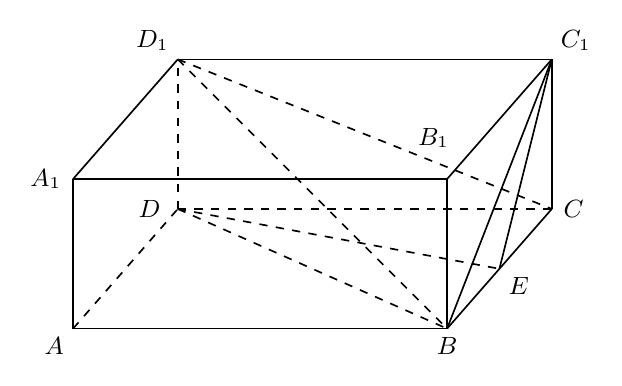
\begin{tikzpicture}[scale=.95,line width=.6pt]
\tikzset{lbl/.style={font=\small,inner sep=1pt}}
\coordinate (A) at (0,0);
\coordinate (B) at (5,0);
\coordinate (C) at (6.4,1.6);
\coordinate (D) at (1.4,1.6);
\coordinate (A1) at (0,2);
\coordinate (B1) at (5,2);
\coordinate (C1) at (6.4,3.6);
\coordinate (D1) at (1.4,3.6);
\coordinate (E) at (5.7000000000,0.8000000000);
% solid
\draw (A)--(B);
\draw (B)--(B1);
\draw (A1)--(B1);
\draw (A)--(A1);
\draw (D1)--(C1);
\draw (C1)--(B);
\draw (C1)--(E);
\draw (B)--(C);\draw (C)--(C1);
% dashed hidden
\draw[dashed] (A)--(D);
\draw[dashed] (D)--(C);
\draw[dashed] (D)--(D1);
\draw (A1)--(D1);
\draw (B1)--(C1);
\draw[dashed] (D1)--(B);

\draw[dashed] (D)--(B);

\draw[dashed] (D1)--(C);
\draw[dashed] (D)--(E);
\node[lbl,below left=2pt] at (A) {$A$};
\node[lbl,below=2pt] at (B) {$B$};
\node[lbl,right=3pt] at (C) {$C$};
\node[lbl,left=5pt] at (D) {$D$};
\node[lbl,left=3pt] at (A1) {$A_{1}$};
\node[lbl,above left=3pt,xshift=5pt,yshift=7pt] at (B1) {$B_{1}$};
\node[lbl,above right=2pt] at (C1) {$C_{1}$};
\node[lbl,above left=2pt] at (D1) {$D_{1}$};
\node[lbl,below right=2pt] at (E) {$E$};
\end{tikzpicture}